Nous avions principalement deux points à respecter : le jeu d'instructions et la présence d'un pipeline à 5 niveaux.

\subsection{Le jeu d’instructions}

Le jeu d'instructions proposé est orienté registre. La présence de \texttt{LOAD} et \texttt{STORE} indique qu'il s'agit d'un processeur RISC LOAD/STORE. Les intructions sont de taille fixe, toutes codées sur 32 bits sous le format suivant : \textbf{A  CodeOP  B  C} (8 bits pour A, 8 bits pour le code opération, 8 bits pour B et 8 bits pour C). Nous n'utiliseront pas forcément tous les octets pour coder une instruction. Pour certaines opérations simples comme le saut inconditionnel, 2 octets suffiront et les 2 restants constitueront du \textit{padding}. La figure \ref{tab:instructions-proc} détaille le jeu d'instruction du processeur.

\begin{table}[h!]
  \centering
  \begin{tabular}{| l | l | l | l |}
    \hline
    Addition & \texttt{0x01} & \texttt{ADD  R$_{X}$  R$_{Y}$  R$_{Z}$} & \texttt{R$_{X}$ $\leftarrow$ R$_{Y}$ $+$ R$_{Z}$} \\ \hline
    Soustraction & \texttt{0x03} & \texttt{SUB  R$_{X}$  R$_{Y}$  R$_{Z}$} & \texttt{R$_{X}$ $\leftarrow$ R$_{Y}$ $-$ R$_{Z}$} \\ \hline
    Multiplication & \texttt{0x02} & \texttt{MUL  R$_{X}$  R$_{Y}$  R$_{Z}$} & \texttt{R$_{X}$ $\leftarrow$ R$_{Y}$ $*$ R$_{Z}$} \\ \hline
    Division (non gérée) & \texttt{0x04} & \texttt{DIV  R$_{X}$  R$_{Y}$  R$_{Z}$} & \texttt{R$_{X}$ $\leftarrow$ R$_{Y}$ $/$ R$_{Z}$} \\ \hline \hline
    Inférieur & \texttt{0x07} & \texttt{INF R$_{X}$  R$_{Y}$  R$_{Z}$} & \texttt{R$_{X}$ $\leftarrow$ R$_{Y}$ $<$ R$_{Z}$} \\ \hline
    Supérieur & \texttt{0x08} & \texttt{SUP R$_{X}$  R$_{Y}$  R$_{Z}$} & \texttt{R$_{X}$ $\leftarrow$ R$_{Y}$ $>$ R$_{Z}$} \\ \hline
    Égal & \texttt{0x09} & \texttt{EQU R$_{X}$  R$_{Y}$  R$_{Z}$} & \texttt{R$_{X}$ $\leftarrow$ R$_{Y}$ $=$ R$_{Z}$} \\ \hline
    Saut inconditionnel & \texttt{0x05} & \texttt{JMP Val$_{saut}$} & \texttt{PC $\leftarrow$ PC $+$ Val$_{saut}$} \\ \hline
    Saut conditionnel & \texttt{0x06} & \texttt{JMF R$_{cond}$  Val$_{saut}$} & \texttt{PC $\leftarrow$ PC $+$ Val$_{saut}$}\\
     & & & quand \texttt{R$_{cond}$ $=$ 0 (false)} \\ \hline \hline
    Copie & \texttt{0x0b} & \texttt{COP  R$_{X}$  R$_{Y}$} & \texttt{R$_{X}$ $\leftarrow$ R$_{Y}$} \\ \hline
    Affectation & \texttt{0x0c} & \texttt{AFC  R$_{X}$  Val} & \texttt{R$_{X}$ $\leftarrow$ Val} \\ \hline
    Chargement & \texttt{0x0d} & \texttt{LOAD  R$_{X}$  Addr$_{orig}$} & \texttt{R$_{X}$ $\leftarrow$ [Addr$_{orig}$]} \\ \hline 
    Sauvegarde & \texttt{0x0e} & \texttt{STORE  Addr$_{dest}$  R$_{X}$} & \texttt{[Addr$_{dest}$] $\leftarrow$ R$_{X}$ }\\ \hline \hline
    Affichage sur l'afficheur 7 segments & \texttt{0x0a} & \texttt{PRI  R$_{X}$} &  \\ \hline \hline
    No Operation & \texttt{0x00} & \texttt{NOP} & \\
    \hline
  \end{tabular}

  

  \caption{Jeu d'instructions}
  \label{tab:instructions-proc}
\end{table}

Comme vous avez certainement pu le noter, nous n'avons pas eu à implémenter toutes les instructions de comparaison de base comme $\neq$, $\leq$, $\geq$ ou logiques comme \texttt{NOT}, \texttt{AND}, \texttt{OR} ou encore \texttt{XOR}. Il en est de même pour les sauts, nous avons un saut inconditionnel et un saut conditionnel qui saute lorsque la condition est fausse.\\
En fait, ces instructions étaient suffisantes et allaient composer les briques pour des opérations plus complexes. Plus d'explications à ce sujet seront données dans la partie liée au compilateur.

\subsection{L'architecture du microprocesseur RISC}

Le microprocesseur est composé d'une unité arithmétique et logique, d'un banc de 16 registres, d'une unité de contrôle de saut, d'une unité de contrôle des aléas, d'une architecture pipeline sur 5 étages, d'une mémoire d'instruction (la ROM), d'une mémoire de données (la RAM) et d'un chemin de données (voir fig.\ref{archi-processeur}).

\begin{figure}[!h]
    \centering
    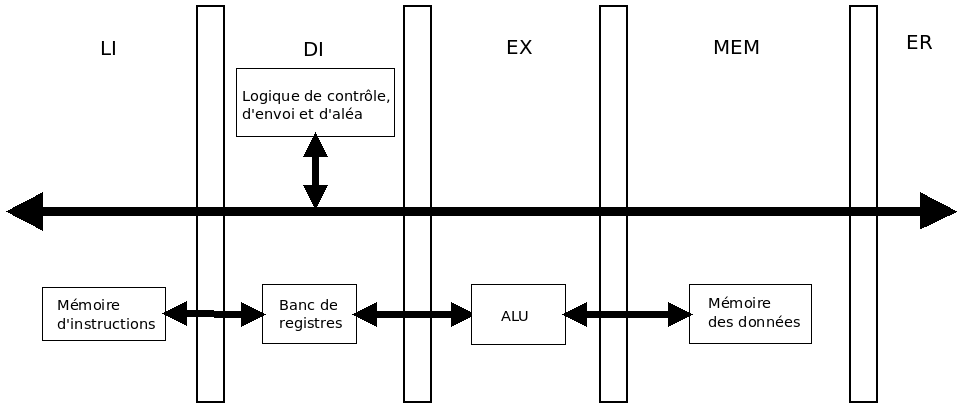
\includegraphics[scale=0.40]{archi-processeur.png}
    \caption{Architecture du processeur RISC}
    \label{archi-processeur}
\end{figure}

\subsubsection*{L'unité arithmétique et logique}

L'ALU effectue les opérations sur des mots de 8 bits. Les 4 bits de contrôle permettent de choisir l'opération à exécuter. Nous avons dû réfléchir à quel moment mettre à jour les flags qui serviront plus tard au saut conditionnel. À chaque opération, le flag \textbf{N} se met à jour en récupérant directement le bit de poids fort du résultat. Quant au flag \textbf{Z}, il passe à un si le résulat est égal à zéro. Le résultat de l'addition, la soustraction et la division tienne sur 8 bits sauf lorsqu'une retenue s'est propagée et celle-ci devient le flag \textbf{C}. Pour terminer, l'\textit{overflow} ne se produit que lorsqu'on a les cas énumérés dans le tableau ci-dessous (fig.\ref{tab:overflow-cases}). Lorsqu'on multiplie deux nombres de 8 bits, le résultat peut tenir sur 16 bits au maximum. Il faudra donc regarder pour le bit de signe le bit 15 alors que pour les autres opérations, ce sera le bit 7. De plus, lors d'une multiplication, tout dépassement au-delà de 8 bits doit être interprété comme un \textit{overflow} car le résultat renvoyé est sur 8 bits.

\begin{table}[h!]
  \centering
  \begin{tabular}{| l | c | c | c |}
    \hline
    Opération & Opérande A (bit 7) & Opérande B (bit 7) & Résultat (bit 7 pour $+$, $-$ et $/$) \\
    & & & et bit 15 pour $*$) \\ \hline
    addition & $\oplus$ & $\oplus$ & $\ominus$ \\ \hline
    addition & $\ominus$ & $\ominus$ & $\oplus$ \\ \hline
    soustraction & $\oplus$ & $\ominus$ & $\ominus$ \\ \hline
    soustraction & $\ominus$ & $\oplus$ & $\oplus$ \\ \hline
    multiplication & $\ominus$ & $\ominus$ & $\ominus$ \\ \hline
    multiplication & $\ominus$ & $\oplus$ & $\oplus$ \\ \hline
    multiplication & $\oplus$ & $\ominus$ & $\oplus$ \\ \hline
    multiplication & $\oplus$ & $\oplus$ & $\ominus$ \\ \hline
    division & $\ominus$ & $\ominus$ & $\ominus$ \\ \hline
    division & $\ominus$ & $\oplus$ & $\oplus$ \\ \hline
    division & $\oplus$ & $\ominus$ & $\oplus$ \\ \hline
    division & $\oplus$ & $\oplus$ & $\ominus$ \\ \hline
  \end{tabular}
  \caption{Énumération des cas d'\textit{overflow} pour les opérations arithmétiques}
  \label{tab:overflow-cases}
\end{table}

\subsubsection*{Le banc de registres}

Il s'agit d'un banc de registres à double port de lecture composé de registres de 8 bits avec accès en lecture et en écriture.

\subsubsection*{Les bancs de mémoire}

La ROM et la RAM ressemblent beaucoup au banc de registres. Nous y reviendrons plus tard pour parler de certaines difficultés dues à notre première implémentation de ces modules.

\subsubsection*{Le chemin de données}

Le chemin de données s'est constitué au fur et à mesure que l'on a intégré les modules. Reprenons le schéma de la figure \ref{archi-processeur} pour suivre le chemin d'une instruction et y voir plus clair. La première étape a consisté à créer les 4 regisres LI, DI, EX, MEM et ER. Il faut ensuite articuler toute la logique de contrôle autour de ces 4 registres.\\

Le premier étage consiste au chargement (\textit{fetch}) de l'instruction présente dans la ROM à l'adresse pointé par le PC (pointeur sur la prochaine instruction). Nous avons créé un registre accueillant la valeur du PC à part du banc de registre alors que l'idéal après recul, aurait été d'utiliser un registre particulier dans le banc et de le consacrer à contenir la valeur du PC. Il en aurait été de même si nous avions implémenté les instructions \texttt{PUSH} et \texttt{POP}, il aurait fallu un autre registre dans le banc pour garder le pointeur de sommet de pile. C'est à partir de cet étage qu'on va injecter les \texttt{NOP} lors d'un aléa.\\

Le deuxième étage va permettre de récupérer la valeur des registres opérandes si l'opération le nécessite. Il existe deux cas particuliers : l'instruction d'affichage \texttt{PRI} et les sauts \texttt{JMP} et \texttt{JMF}.\\
Le contenu du registre spécifié par \texttt{PRI} est chargé dans un registre interne au processeur que le  contrôleur de l'afficheur 7 segments va venir lire avec une fréquence de 1KHz pour ensuite aller afficher sa valeur en hexadécimal.\\
En ce qui concerne les sauts, on va aller récupérer la valeur du PC et la charger dans la partie C de l'instruction qui n'était jusqu'à présent pas utilisée. Cette valeur va être utilisée au niveau de l'ALU afin de calculer la nouvelle valeur du PC.\\
 
Le troisième étage consiste à récupérer le sortie de l'ALU et recupérer également la valeur des flags selon l'opération.\\

Le quatrième étage permet de stocker ou récupérer une valeur à une adresse de la RAM. Un multiplexeur asynchrone permet de choisir la bonne partie de l'opération à passer en adresse et en donnée à la RAM.\\

Le cinquième étage a pour charge d'affecter les registres. Il est composée lui aussi d'un multiplexeur et est très semblable au quatrième étage.